\documentclass[twocolumn]{article}
\usepackage{amsmath}
\usepackage{graphicx}
\usepackage{hyperref}
\title{Reversible Modular Addition using a Dirty Bit}
\author{Craig Gidney}

\begin{document}
\maketitle

\begin{abstract}
\em
We present reversible classical circuits for performing addition, incrementation, comparisons, modular addition, and modular offset on registers of differing sizes using no ancilla or 1 ancilla in an unknown state.
We improve the best known space requirements for factoring an $n$-bit number from $2n+2$ qubits to $2n+1$ qubits, without increasing the asymptotic depth or size of the circuit.
\end{abstract}

\section{Introduction}

When constructing quantum circuits, or classical reversible circuits, an important resource is the number of available ancilla.
An ancilla is an extra bit or qubit, on top of those used for input and output, available for use as temporary workspace.
Ancilla may be initialized to a known state (``clean bit"), or be given to the circuit in an unknown state (``dirty bit") that must be restored before the circuit finishes.
Clean bits are more valuable, allowing for simpler and more compact circuit constructions, but dirty bits are more plentiful, because any temporarily unused qubit is a borrowable dirty bit.

The ability for part of a circuit to borrow dirty bits from another part of the same circuit makes circuit constructions that require only dirty bits very flexible.
Especially in situations with space constraints, or on circuit topologies where clean ancilla are too far away to be acquired quickly.
For example, \cite{haner2016} improves the cost of performing Shor's algorithm, when limited to using only $2n+2$ qubits, to $O(n^3)$ depth and $O(n^3 \lg n)$ size by introducing an offset gate that borrows dirty bits from one register while offsetting the other.
We improve on \cite{haner2016} by cutting the number of required qubits from $2n+2$ to $2n+1$.

The paper is structured as follows.
The introduction describes the various sections and also itself for no discernible reason.
Section \ref{sec:review} discusses existing circuit constructions.
In sections \ref{sec:first-circuit} through \ref{sec:last-circuit} we describe our various arithmetic circuit constructions.
Section \ref{sec:applications} discusses how to use our constructions to factor an $n$ bit number using $2n+1$ qubits.
Section \ref{sec:conclusion} concludes.

All constructions assume a 2s-complement representation of integers.
All circuit diagrams with multi-wire integer operations put the least significant bit towards the top.

\section{Existing Constructions} \label{sec:review}

\subsection{Addition}

\cite{draper2000} describes an addition circuit that uses the quantum Fourier transform to convert phasing into shifting.
Their naive construction uses $O(N)$ depth and $O(N^2)$ controlled rotations, but this can be improved to $O(\lg N)$ depth and $O(N \lg N)$ size by using approximation techniques \cite{barenco1996} \cite{cleve2000}.

\cite{cuccaro2004} and \cite{van2004} describe classical reversible adders that use a single clean ancilla, $O(N)$ depth, and $O(N)$ size.

\cite{takahashi2005} and \cite{takahashi2009} describe classical reversible adders that use no ancilla.

We improve on \cite{takahashi2005} by allowing addition into larger registers.

\subsection{Offset}

An offset gate adds a compile-time constant into a register.
Many reversible adder constructions do not work in this case because there is no input register to use as temporary workspace.

\cite{draper2000}'s QFT-based addition doesn't need the source register as workspace, and so can be applied to this problem.

\cite{haner2016} describes a divide-and-conquer offset circuit that requires $O(N)$ depth, $O(N \lg N)$ size, and $1$ dirty ancilla (or 0 if using quantum operations).

This paper describes a circuit for the special case of offset-by-1, i.e. incrementation, that uses $O(N)$ depth and size and a single dirty ancilla.
We also show how to remove the ancilla with quantum operations.
The construction is a simplified version of the incrementer described in \cite{gidney2015}.

\subsection{Comparison}

\cite{takahashi2005} describes inline comparison operations.
We improve on this construction by allowing the comparison of registers of different sizes.

\subsection{Modular Addition}

\cite{vedral1995} describes a modular adder that uses $O(N)$ clean ancilla, based on performing normal addition and subtraction and temporarily storing a comparison in a clean ancilla.
Most of the clean ancilla are only used for the addition and subtraction, so using inline adders reduces the number of clean ancilla required to 1, as used in \cite{haner2016}.

We improve on this construction by allowing the ancilla to be dirty.

\section{$O(N)$ inline adders} \label{sec:first-circuit}

[[[ Should I cut most of this? Cited papers do just as well. ]]]

In \cite{van2004}, a reversible adder with $O(N)$ depth and $O(N)$ size, requiring a single clean ancilla, is described.
If the ancilla is not initialized in the off state, the target register ends up storing $a+b+1$ instead of $a+b$.

The need for the ancilla to be clean can be fixed by inverting (bitwise-NOT-ing) the source and target registers before and after the addition when the ancilla is on.
Because $\lnot x = -x-1$, and the registers are the same size, temporarily inverting the target effectively turns the addition into a subtraction.
Temporarily inverting the source turns the subtraction back into an addition, but also introduces an extra shift by -1, cancelling out the +1 error.

On top of allowing the ancilla to be dirty, the ancilla's role can be merged into the most-significant-bit (MSB) of the source register as shown in figure \ref{fig:inlineadder}.

\begin{figure}
  \centering
  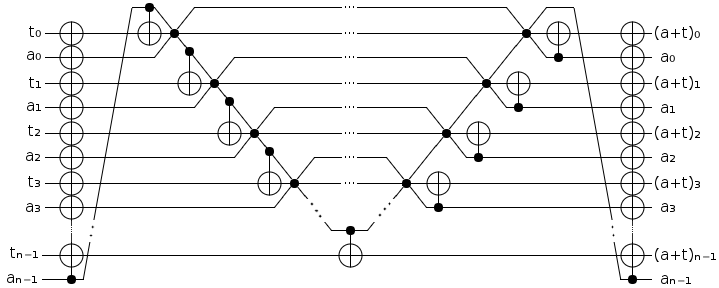
\includegraphics[totalheight=3cm]{inline-adder.png}
  \caption{\em Same-register-size adder using no ancilla, $6N-3$ CNOTs, and $2N-2$ CSWAPs. Based on \cite{van2004}.}
  \label{fig:inlineadder}
\end{figure}

To perform subtraction instead of addition: run the circuit in reverse, temporarily invert the target register by bordering the circuit with NOT gates on the target, or invert the CSWAP controls.

Because the source register is used as workspace, the construction in figure \ref{fig:inlineadder} only works when the source register is the same size as the target register.
When the source register is larger, the issue is easily avoided by ignoring the high bits of the source register.
When the target register is larger, the workaround is more difficult.
Not only is there insufficient workspace, but the register sizes being different breaks the logical-negation trick that allowed the carry signalling bit to be dirty.

The problems caused by the target register being larger can be overcome by using the increment and decrement constructions from the next section.
(Note that they use only the same-register-size adder, not the adder about to be defined.)
The carry signal can be forwarded into the high part of the target register with a controlled increment.
The MSB of the source register can be free'd for use as a borrowed dirty bit by performing the MSB's controlled increment.
Finally, the extra increment caused by the borrowed dirty bit being on can be cancelled with a controlled decrement.
See the circuit diagram in figure \ref{fig:inline-adder-into-large}.

\begin{figure}
  \centering
  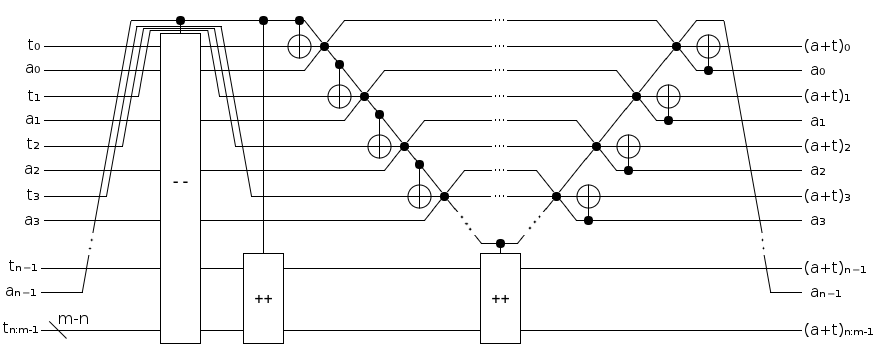
\includegraphics[totalheight=3cm]{inline-adder-into-large.png}
  \caption{\em
      Adder with target larger than source, using no ancilla.
      Uses increment constructions that use the same-size adder.}
  \label{fig:inline-adder-into-large}
\end{figure}

\section{$O(N)$ incrementer}

A register can be incremented by subtracting both $x$ and $\neg x = -x-1$ from it, for any $x$.
When $N$ dirty bits are available, $x$ can come from the register defined by those $N$ bits, as shown in figure \ref{fig:double-sub-increment}.

\begin{figure}
  \centering
  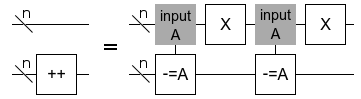
\includegraphics[totalheight=2cm]{double-sub-increment.png}
  \caption{\em Subtracting $x$ and $-x-1$ from a register increments it. Requires $O(N)$ depth, size, and $N$ dirty ancilla.}
  \label{fig:double-sub-increment}
\end{figure}

To improve from $N$ dirty bits to a single dirty bit, we break the increment operation into two halves.
A top half that is incremented only if all of the bottom bits are on, and a bottom half that is unconditionally incremented.
The bottom half can be incremented with the double-subtraction trick by borrowing the top half.
But the trick doesn't work on the top half, because the bottom half can't be borrowed when it is being used as a control.

To work around not being able to operate on the borrowed bits while using them as a control, start with the double-subtraction trick but change the second subtraction to an addition and conditionally toggle the target bits instead of the input bits.
When the condition isn't satisfied, the addition and subtraction will cancel each other.
When the condition is satisfied, the addition is inverted into a subtraction.
Both the subtraction and addition-turned-subtraction fire, subtracting the input register from the target register twice.
However, because we are conditioning on the input bits all being on, the input must be -1.
Therefore the target was incremented by 2.
To halve the +2 into a +1, prepend a dirty LSB onto the target register as shown in \ref{fig:compact-increment}.

\begin{figure}
  \centering
  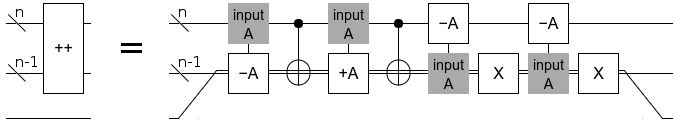
\includegraphics[totalheight=1.5cm]{compact-increment.png}
  \caption{\em Odd-sized $O(N)$ increment with 1 dirty ancilla.}
  \label{fig:compact-increment}
\end{figure}

Because the adder/subtracter construction used by the incrementer in figure \ref{fig:compact-increment} requires the target and source registers to be the same size, the construction only works on odd-sized registers.
For even-sized registers, another minor variation on the conditionally-invert-addition-into-subtraction-with-logical-negation technique is used.
The construction is shown in figure \ref{fig:compact-increment-even}.

\begin{figure}
  \centering
  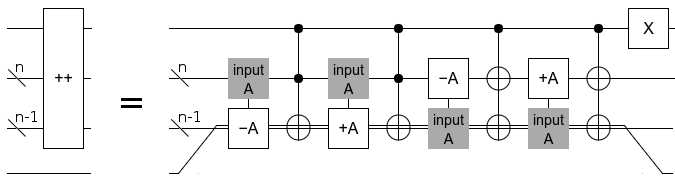
\includegraphics[totalheight=2cm]{compact-increment-even.png}
  \caption{\em Even-sized $O(N)$ increment with 1 dirty ancilla.}
  \label{fig:compact-increment-even}
\end{figure}

As with addition and subtraction, you can turn an increment into a decrement either by reversing the gate order, by bordering the circuit with NOT gates, or by inverting all of the controls.
Also, increment gates can be controlled by using another invert-input-and-output trick (see figures \ref{fig:controlled-increment-odd} and \ref{fig:controlled-increment-even}).

\begin{figure}
  \centering
  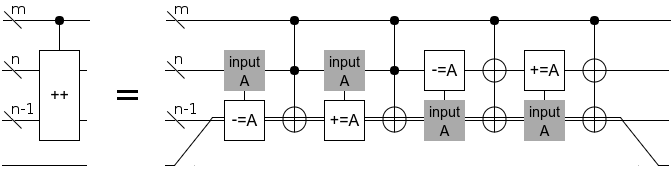
\includegraphics[totalheight=2cm]{controlled-increment-odd.png}
  \caption{\em Odd-sized $O(N)$ controlled increment with 1 dirty ancilla.}
  \label{fig:controlled-increment-odd}
\end{figure}

\begin{figure}
  \centering
  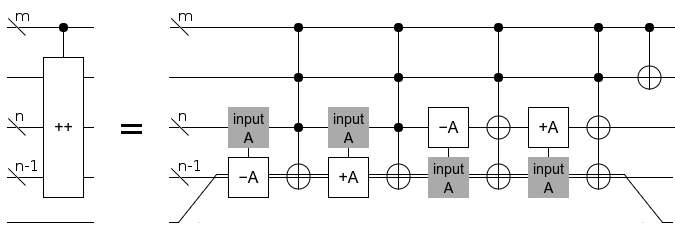
\includegraphics[totalheight=2.5cm]{controlled-increment-even.png}
  \caption{\em Even-sized $O(N)$ controlled increment with 1 dirty ancilla.}
  \label{fig:controlled-increment-even}
\end{figure}

Note that, unlike with register-to-register addition, it is impossible to create a classical incrementer that uses no ancilla.
The parity of the permutation performed by an increment operation is odd, but the parity of the permutation performed by any classical gate that doesn't cover the entire circuit is even.
Quantumly, the parity barrier can be bypassed by using partial rotations (see figure \ref{fig:bootstrap-ancilla}).

\begin{figure}
  \centering
  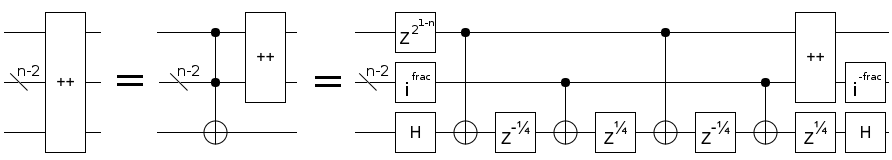
\includegraphics[totalheight=1.4cm]{ancilla-bootstrap.png}
  \caption{\em Bootstrapping dirty ancilla out of an increment gate using quantum operations.
  The $i^{\text{frac}}$ operation is implemented by a column of $Z^{2^{-k}}$ gates.
  The 'frac' refers to the fraction $v/2^d$, where $v$ is the computational-basis value in the register and $d$ is the size of the register.}
  \label{fig:bootstrap-ancilla}
\end{figure}

\section{$O(N)$ inline comparisons}

Comparison operations toggle a target bit based on the relationship between two input registers.

The is-B-less-than-A comparison is implemented by subtracting $A$ out of $B$ with the target bit appended to $B$, then adding $A$ into $B$ without the target bit appended.
See figure \ref{fig:comparison-less}.

\begin{figure}
  \centering
  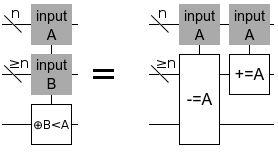
\includegraphics[totalheight=3cm]{comparison-less.png}
  \caption{\em Toggling a target bit if one register is less than another, without using ancilla.}
  \label{fig:comparison-less}
\end{figure}

The same idea is used for is-B-less-than-or-equal-to-A, except $A+1$ is subtracted and added instead of $A$.
The extra $\pm 1$ is performed by increment and decrement gates, as shown in figure \ref{fig:comparison-leq}.
When the two registers are the same size, the increment gate can be omitted by inverting the $A$ and $B$ registers during the addition.

$>$ and $\geq$ comparisons are done by performing the opposite comparison ($\leq$ and $<$ respectively) and inverting the result by toggling the target.
To perform a comparison when the $B$ register is smaller than the $A$ register, swap their roles and use the opposite comparison.

\begin{figure}
  \centering
  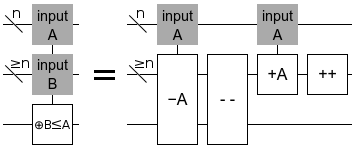
\includegraphics[totalheight=3cm]{comparison-leq.png}
  \caption{\em Toggling a target bit if one register is less than or equal to another, without using ancilla.}
  \label{fig:comparison-leq}
\end{figure}

\section{$\text{PivotFlip}$}

A pivot-flip operation reverses the order of states less than or equal to a given pivot value.
For example, a pivot-flip with the pivot equal to 3 would swap $|0\rangle$ and $|3\rangle$, swap $|1\rangle$ and $|2\rangle$, and leave all other states untouched.
Pivot-flips are useful for implementing cyclic operations, such as modular addition.

The exact permutation performed by a pivot-flip with pivot equal to $k$ is:

$$\text{PivotFlip}_k = \sum_{i=0}^k |k-i\rangle \langle i| + \sum_{i=k+1}^{N-1} |i\rangle \langle i|$$

And the overall permutation, including the pivot input, is:

$$\text{PivotFlip} = \sum_{k=0}^{N-1} |k\rangle \langle k| \otimes \text{PivotFlip}_{k}$$

To perform a pivot-flip efficiently, we use the fact that $x \rightarrow \lnot(x + \lnot a)$ nearly does what is required.
As shown in figure \ref{fig:double-flip}, the permutation $x \rightarrow \lnot(x + \lnot a)$ flips the range below-and-including the pivot but also flips the range above the pivot.
However, because $x \rightarrow \lnot(x + \lnot a)$ is its own inverse and doesn't change whether any value is less than or equal to the pivot, the operation can be restricted by dirty comparisons against the pivot.

By applying $x \rightarrow \lnot(x + \lnot a)$ twice, controlled by a dirty bit that is toggled by the comparison, the desired effect is achieved.
For states that are less than or equal to $A$, only one of the controlled flips happens.
For other states, the controlled flip happens no times or two times, undoing itself.
See figure \ref{fig:const-pivot-flip}, which also includes a variant for pivot-flipping while excluding the pivot.

\begin{figure}
  \centering
  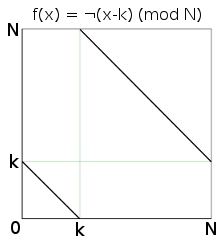
\includegraphics[totalheight=4cm]{double-flip.png}
  \caption{\em Subtraction followed by logical negation performs flips both above and below $k$.}
  \label{fig:double-flip}
\end{figure}

\begin{figure}
  \centering
  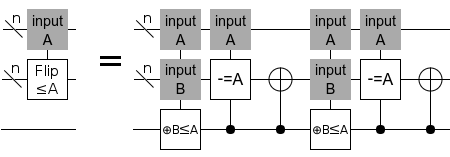
\includegraphics[totalheight=4.5cm]{pivot-flip.png}
  \caption{\em Pivot flip circuits.
  When the top wire bundle is a register, the subtractions are controlled by replacing the CNOTs in figure \ref{fig:inlineadder} with CCNOTs.
  When the top wire bundle is a compile-time constant, the subtractions use the construction from \cite{haner2016} and are controlled as shown in figure \ref{fig:controlled-offset}.}
  \label{fig:const-pivot-flip}
\end{figure}

\begin{figure}
  \centering
  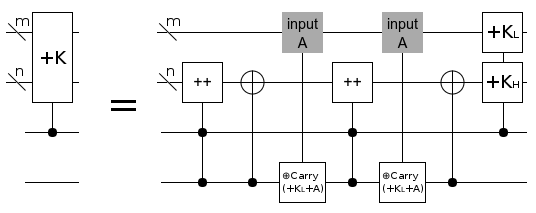
\includegraphics[totalheight=3.1cm]{controlled-offset.png}
  \caption{\em Offset circuit from \cite{haner2016}, modified to include a control.}
  \label{fig:controlled-offset}
\end{figure}

The cost of a $\text{PivotFlip}$ depends on if the pivot is a compile-time constant or not.
When the pivot is input from another register, the $O(N)$ inline adder can be used.
But when the pivot is a constant, the $O(N \lg N)$ size and $O(N)$ depth offset gate from \cite{haner2016} is used instead.

\section{$O(N \lg N)$ Modular Addition and Modular Offset} \label{sec:last-circuit}

A modular addition is three pivot flips.
To add $a$ into a register modulo $r$, perform pivot-flips with the pivot at $r-1-a$, then $r-1$, then $a-1$.
See figure \ref{fig:modular-add}.

\begin{figure}
  \centering
  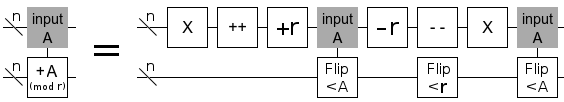
\includegraphics[totalheight=1.4cm]{modular-addition.png}
  \caption{\em Modular addition circuit.
  The $+r$ offset gates require $O(N \lg N)$ size.
  The pivot-flips require a dirty bit.}
  \label{fig:modular-add}
\end{figure}

Note that we have implemented modular addition in terms of normal addition.
This fact is obfuscated by the number of constructions used but, as shown in figure \ref{fig:modular-dependencies}, addition and offset (constant addition) are the only operations not defined in terms of another operations.

\begin{figure}
  \centering
  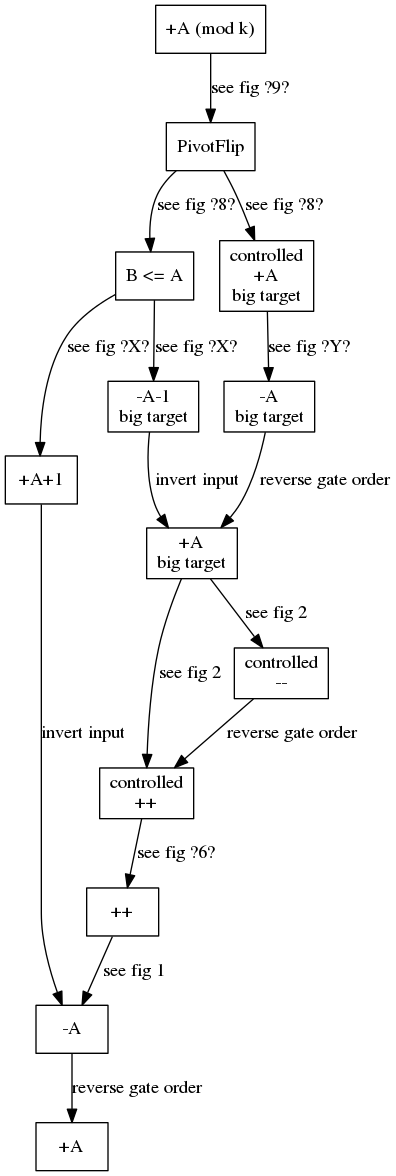
\includegraphics[totalheight=16cm]{modular-add-graph.png}
  \caption{\em
      Dependency graph of constructions used to create a classical reversible modular adder / modular offset gates using only 1 dirty bit.}
  \label{fig:modular-dependencies}
\end{figure}

\section{Factoring with $2n+1$ qubits} \label{sec:applications}

\cite{haner2016} describes how to perform Shor's algorithm with Toffoli-based circuits using $2n+2$ qubits.
The first $n$ qubits are needed to hold the input.
The second $n$ qubits are for holding the output of exponentiating the input modulo a constant.
One of the remaining qubits is used for the phase estimation process.
The last qubit is a clean ancilla used by modular addition.

The modular addition circuit we have presented does not require a clean ancilla.
The need for the last ancilla is avoided by instead borrowing the phase estimation qubit as a temporary dirty bit.

[[[What about underlying details I didn't mention, like reducing many-controlled many-nots?]]]

[[[ Maybe some more details...? ]]]

\section{Conclusion} \label{sec:conclusion}

[[[TODO]]]

\bibliographystyle{plain}
\bibliography{citations}

\section{Test Circuit Links}

Convenience links for myself when checking that things work.

\href
{http://algassert.com/quirk#circuit=%7B%22cols%22%3A%5B%5B%22X%22%2C%22X%22%2C%22X%22%2C%22X%22%2C%22%E2%80%A2%22%2C%22X%22%2C%22X%22%2C%22X%22%2C%22X%22%2C%22X%22%5D%2C%5B%22%E2%80%A2%22%2C1%2C1%2C1%2C1%2C%22X%22%5D%2C%5B%22Swap%22%2C1%2C1%2C1%2C%22Swap%22%2C%22%E2%80%A2%22%5D%2C%5B1%2C%22%E2%80%A2%22%2C1%2C1%2C1%2C1%2C%22X%22%5D%2C%5B1%2C%22Swap%22%2C1%2C1%2C%22Swap%22%2C1%2C%22%E2%80%A2%22%5D%2C%5B1%2C1%2C%22%E2%80%A2%22%2C1%2C1%2C1%2C1%2C%22X%22%5D%2C%5B1%2C1%2C%22Swap%22%2C1%2C%22Swap%22%2C1%2C1%2C%22%E2%80%A2%22%5D%2C%5B1%2C1%2C1%2C%22%E2%80%A2%22%2C1%2C1%2C1%2C1%2C%22X%22%5D%2C%5B1%2C1%2C1%2C%22Swap%22%2C%22Swap%22%2C1%2C1%2C1%2C%22%E2%80%A2%22%5D%2C%5B1%2C1%2C1%2C1%2C%22%E2%80%A2%22%2C1%2C1%2C1%2C1%2C%22X%22%5D%2C%5B1%2C1%2C1%2C%22Swap%22%2C%22Swap%22%2C1%2C1%2C1%2C%22%E2%80%A2%22%5D%2C%5B1%2C1%2C1%2C1%2C%22%E2%80%A2%22%2C1%2C1%2C1%2C%22X%22%5D%2C%5B1%2C1%2C%22Swap%22%2C1%2C%22Swap%22%2C1%2C1%2C%22%E2%80%A2%22%5D%2C%5B1%2C1%2C1%2C1%2C%22%E2%80%A2%22%2C1%2C1%2C%22X%22%5D%2C%5B1%2C%22Swap%22%2C1%2C1%2C%22Swap%22%2C1%2C%22%E2%80%A2%22%5D%2C%5B1%2C1%2C1%2C1%2C%22%E2%80%A2%22%2C1%2C%22X%22%5D%2C%5B%22Swap%22%2C1%2C1%2C1%2C%22Swap%22%2C%22%E2%80%A2%22%5D%2C%5B1%2C1%2C1%2C1%2C%22%E2%80%A2%22%2C%22X%22%5D%2C%5B%22X%22%2C%22X%22%2C%22X%22%2C%22X%22%2C%22%E2%80%A2%22%2C%22X%22%2C%22X%22%2C%22X%22%2C%22X%22%2C%22X%22%5D%5D%7D}
{5+5-bit inline adder}
(or \href
{http://algassert.com/quirk#circuit=%7B%22cols%22%3A%5B%5B%22Counting10%22%5D%2C%5B%22QFT7%22%5D%2C%5B1%2C1%2C1%2C%22QFT7%22%5D%2C%5B%22%E2%80%A6%22%5D%2C%5B%22%E2%80%A6%22%5D%2C%5B%22X%22%2C%22X%22%2C%22X%22%2C%22X%22%2C%22%E2%80%A2%22%2C%22X%22%2C%22X%22%2C%22X%22%2C%22X%22%2C%22X%22%5D%2C%5B%22%E2%80%A2%22%2C1%2C1%2C1%2C1%2C%22X%22%5D%2C%5B%22Swap%22%2C1%2C1%2C1%2C%22Swap%22%2C%22%E2%80%A2%22%5D%2C%5B1%2C%22%E2%80%A2%22%2C1%2C1%2C1%2C1%2C%22X%22%5D%2C%5B1%2C%22Swap%22%2C1%2C1%2C%22Swap%22%2C1%2C%22%E2%80%A2%22%5D%2C%5B1%2C1%2C%22%E2%80%A2%22%2C1%2C1%2C1%2C1%2C%22X%22%5D%2C%5B1%2C1%2C%22Swap%22%2C1%2C%22Swap%22%2C1%2C1%2C%22%E2%80%A2%22%5D%2C%5B1%2C1%2C1%2C%22%E2%80%A2%22%2C1%2C1%2C1%2C1%2C%22X%22%5D%2C%5B1%2C1%2C1%2C%22Swap%22%2C%22Swap%22%2C1%2C1%2C1%2C%22%E2%80%A2%22%5D%2C%5B1%2C1%2C1%2C1%2C%22%E2%80%A2%22%2C1%2C1%2C1%2C1%2C%22X%22%5D%2C%5B1%2C1%2C1%2C%22Swap%22%2C%22Swap%22%2C1%2C1%2C1%2C%22%E2%80%A2%22%5D%2C%5B1%2C1%2C1%2C1%2C%22%E2%80%A2%22%2C1%2C1%2C1%2C%22X%22%5D%2C%5B1%2C1%2C%22Swap%22%2C1%2C%22Swap%22%2C1%2C1%2C%22%E2%80%A2%22%5D%2C%5B1%2C1%2C1%2C1%2C%22%E2%80%A2%22%2C1%2C1%2C%22X%22%5D%2C%5B1%2C%22Swap%22%2C1%2C1%2C%22Swap%22%2C1%2C%22%E2%80%A2%22%5D%2C%5B1%2C1%2C1%2C1%2C%22%E2%80%A2%22%2C1%2C%22X%22%5D%2C%5B%22Swap%22%2C1%2C1%2C1%2C%22Swap%22%2C%22%E2%80%A2%22%5D%2C%5B1%2C1%2C1%2C1%2C%22%E2%80%A2%22%2C%22X%22%5D%2C%5B%22X%22%2C%22X%22%2C%22X%22%2C%22X%22%2C%22%E2%80%A2%22%2C%22X%22%2C%22X%22%2C%22X%22%2C%22X%22%2C%22X%22%5D%2C%5B%22%E2%80%A6%22%5D%2C%5B%22%E2%80%A6%22%5D%2C%5B%22inputA5%22%2C1%2C1%2C1%2C1%2C%22%2B%3DA5%22%5D%2C%5B1%2C1%2C1%2C%22QFT%E2%80%A07%22%5D%2C%5B%22QFT%E2%80%A07%22%5D%2C%5B%22Uncounting10%22%5D%5D%7D}
{with test harness})

\href
{http://algassert.com/quirk#circuit=%7B%22cols%22%3A%5B%5B%22inputA4%22%2C1%2C1%2C1%2C%22-%3DA4%22%5D%2C%5B%22X%22%2C%22X%22%2C%22X%22%2C%22X%22%5D%2C%5B%22inputA4%22%2C1%2C1%2C1%2C%22-%3DA4%22%5D%2C%5B%22X%22%2C%22X%22%2C%22X%22%2C%22X%22%5D%5D%7D}
{4-bit incrementer w/ 4 dirty}

\href
{http://algorithmicassertions.com/quirk#circuit=%7B%22cols%22%3A%5B%5B1%2C1%2C1%2C1%2C1%2C%22%3C%3C4%22%5D%2C%5B1%2C%22inputA4%22%2C1%2C1%2C1%2C%22-%3DA4%22%5D%2C%5B%22%E2%80%A2%22%2C%22%E2%80%A2%22%2C%22%E2%80%A2%22%2C%22%E2%80%A2%22%2C%22%E2%80%A2%22%2C%22X%22%2C%22X%22%2C%22X%22%2C%22X%22%5D%2C%5B1%2C%22inputA4%22%2C1%2C1%2C1%2C%22%2B%3DA4%22%5D%2C%5B%22%E2%80%A2%22%2C%22%E2%80%A2%22%2C%22%E2%80%A2%22%2C%22%E2%80%A2%22%2C%22%E2%80%A2%22%2C%22X%22%2C%22X%22%2C%22X%22%2C%22X%22%5D%2C%5B1%2C%22-%3DA4%22%2C1%2C1%2C1%2C%22inputA4%22%5D%2C%5B%22%E2%80%A2%22%2C%22X%22%2C%22X%22%2C%22X%22%2C%22X%22%2C%22X%22%2C%22X%22%2C%22X%22%2C%22X%22%5D%2C%5B1%2C%22%2B%3DA4%22%2C1%2C1%2C1%2C%22inputA4%22%5D%2C%5B%22%E2%80%A2%22%2C%22X%22%2C%22X%22%2C%22X%22%2C%22X%22%2C%22X%22%2C%22X%22%2C%22X%22%2C%22X%22%5D%2C%5B%22X%22%5D%2C%5B1%2C1%2C1%2C1%2C1%2C%22%3E%3E4%22%5D%5D%7D}
{8-bit incrementer w/ 1 dirty}
(or \href
{http://algorithmicassertions.com/quirk#circuit=%7B%22cols%22%3A%5B%5B%22Counting9%22%5D%2C%5B%22QFT6%22%5D%2C%5B1%2C1%2C1%2C%22QFT6%22%5D%2C%5B%22%E2%80%A6%22%5D%2C%5B%22%E2%80%A6%22%5D%2C%5B1%2C1%2C1%2C1%2C1%2C%22%3C%3C4%22%5D%2C%5B1%2C%22inputA4%22%2C1%2C1%2C1%2C%22-%3DA4%22%5D%2C%5B%22%E2%80%A2%22%2C%22%E2%80%A2%22%2C%22%E2%80%A2%22%2C%22%E2%80%A2%22%2C%22%E2%80%A2%22%2C%22X%22%2C%22X%22%2C%22X%22%2C%22X%22%5D%2C%5B1%2C%22inputA4%22%2C1%2C1%2C1%2C%22%2B%3DA4%22%5D%2C%5B%22%E2%80%A2%22%2C%22%E2%80%A2%22%2C%22%E2%80%A2%22%2C%22%E2%80%A2%22%2C%22%E2%80%A2%22%2C%22X%22%2C%22X%22%2C%22X%22%2C%22X%22%5D%2C%5B1%2C%22-%3DA4%22%2C1%2C1%2C1%2C%22inputA4%22%5D%2C%5B%22%E2%80%A2%22%2C%22X%22%2C%22X%22%2C%22X%22%2C%22X%22%2C%22X%22%2C%22X%22%2C%22X%22%2C%22X%22%5D%2C%5B1%2C%22%2B%3DA4%22%2C1%2C1%2C1%2C%22inputA4%22%5D%2C%5B%22%E2%80%A2%22%2C%22X%22%2C%22X%22%2C%22X%22%2C%22X%22%2C%22X%22%2C%22X%22%2C%22X%22%2C%22X%22%5D%2C%5B%22X%22%5D%2C%5B1%2C1%2C1%2C1%2C1%2C%22%3E%3E4%22%5D%2C%5B%22%E2%80%A6%22%5D%2C%5B%22%E2%80%A6%22%5D%2C%5B%22dec8%22%5D%2C%5B1%2C1%2C1%2C%22QFT%E2%80%A06%22%5D%2C%5B%22QFT%E2%80%A06%22%5D%2C%5B%22Uncounting9%22%5D%5D%7D}
{with test harness})

\href
{http://algorithmicassertions.com/quirk#circuit=%7B%22cols%22%3A%5B%5B1%2C1%2C1%2C1%2C1%2C%22%3C%3C5%22%5D%2C%5B%22inputA5%22%2C1%2C1%2C1%2C1%2C%22-%3DA5%22%5D%2C%5B%22%E2%80%A2%22%2C%22%E2%80%A2%22%2C%22%E2%80%A2%22%2C%22%E2%80%A2%22%2C%22%E2%80%A2%22%2C%22X%22%2C%22X%22%2C%22X%22%2C%22X%22%2C%22X%22%5D%2C%5B%22inputA5%22%2C1%2C1%2C1%2C1%2C%22%2B%3DA5%22%5D%2C%5B%22%E2%80%A2%22%2C%22%E2%80%A2%22%2C%22%E2%80%A2%22%2C%22%E2%80%A2%22%2C%22%E2%80%A2%22%2C%22X%22%2C%22X%22%2C%22X%22%2C%22X%22%2C%22X%22%5D%2C%5B%22-%3DA5%22%2C1%2C1%2C1%2C1%2C%22inputA5%22%5D%2C%5B1%2C1%2C1%2C1%2C1%2C%22X%22%2C%22X%22%2C%22X%22%2C%22X%22%2C%22X%22%5D%2C%5B%22-%3DA5%22%2C1%2C1%2C1%2C1%2C%22inputA5%22%5D%2C%5B1%2C1%2C1%2C1%2C1%2C%22X%22%2C%22X%22%2C%22X%22%2C%22X%22%2C%22X%22%5D%2C%5B1%2C1%2C1%2C1%2C1%2C%22%3E%3E5%22%5D%5D%7D}
{9-bit incrementer w/ 1 dirty}
(or \href
{http://algorithmicassertions.com/quirk#circuit=%7B%22cols%22%3A%5B%5B%22Counting10%22%5D%2C%5B%22QFT7%22%5D%2C%5B1%2C1%2C1%2C%22QFT7%22%5D%2C%5B%22%E2%80%A6%22%5D%2C%5B%22%E2%80%A6%22%5D%2C%5B1%2C1%2C1%2C1%2C1%2C%22%3C%3C5%22%5D%2C%5B%22inputA5%22%2C1%2C1%2C1%2C1%2C%22-%3DA5%22%5D%2C%5B%22%E2%80%A2%22%2C%22%E2%80%A2%22%2C%22%E2%80%A2%22%2C%22%E2%80%A2%22%2C%22%E2%80%A2%22%2C%22X%22%2C%22X%22%2C%22X%22%2C%22X%22%2C%22X%22%5D%2C%5B%22inputA5%22%2C1%2C1%2C1%2C1%2C%22%2B%3DA5%22%5D%2C%5B%22%E2%80%A2%22%2C%22%E2%80%A2%22%2C%22%E2%80%A2%22%2C%22%E2%80%A2%22%2C%22%E2%80%A2%22%2C%22X%22%2C%22X%22%2C%22X%22%2C%22X%22%2C%22X%22%5D%2C%5B%22-%3DA5%22%2C1%2C1%2C1%2C1%2C%22inputA5%22%5D%2C%5B1%2C1%2C1%2C1%2C1%2C%22X%22%2C%22X%22%2C%22X%22%2C%22X%22%2C%22X%22%5D%2C%5B%22-%3DA5%22%2C1%2C1%2C1%2C1%2C%22inputA5%22%5D%2C%5B1%2C1%2C1%2C1%2C1%2C%22X%22%2C%22X%22%2C%22X%22%2C%22X%22%2C%22X%22%5D%2C%5B1%2C1%2C1%2C1%2C1%2C%22%3E%3E5%22%5D%2C%5B%22%E2%80%A6%22%5D%2C%5B%22%E2%80%A6%22%5D%2C%5B%22dec9%22%5D%2C%5B1%2C1%2C1%2C%22QFT%E2%80%A07%22%5D%2C%5B%22QFT%E2%80%A07%22%5D%2C%5B%22Uncounting10%22%5D%5D%7D}
{with test harness})

\href
{http://algorithmicassertions.com/quirk#circuit=%7B%22cols%22%3A%5B%5B%22Z%5E%E2%85%9F%E2%82%81%E2%82%86%22%2C%22Z%5E%E2%85%9F%E2%82%81%E2%82%86%22%2C%22Z%5E%E2%85%9B%22%2C%22Z%5E%C2%BC%22%2C%22H%22%5D%2C%5B%22%E2%80%A2%22%2C1%2C1%2C1%2C%22X%22%5D%2C%5B1%2C1%2C1%2C1%2C%22Z%5E-%C2%BC%22%5D%2C%5B1%2C%22%E2%80%A2%22%2C%22%E2%80%A2%22%2C%22%E2%80%A2%22%2C%22X%22%5D%2C%5B1%2C1%2C1%2C1%2C%22Z%5E%C2%BC%22%5D%2C%5B%22%E2%80%A2%22%2C1%2C1%2C1%2C%22X%22%5D%2C%5B1%2C1%2C1%2C1%2C%22Z%5E-%C2%BC%22%5D%2C%5B1%2C%22%E2%80%A2%22%2C%22%E2%80%A2%22%2C%22%E2%80%A2%22%2C%22X%22%5D%2C%5B%22inc4%22%2C1%2C1%2C1%2C%22Z%5E%C2%BC%22%5D%2C%5B1%2C%22Z%5E-%E2%85%9F%E2%82%81%E2%82%86%22%2C%22Z%5E-%E2%85%9B%22%2C%22Z%5E-%C2%BC%22%2C%22H%22%5D%5D%7D}
{Quantum incrementer ancilla bootstrap}

NOTE: have to open these next ones against local version, because online version doesn't have the comparison gates

\href
{http://algassert.com/quirk#circuit=%7B%22cols%22%3A%5B%5B%22inputA4%22%2C1%2C1%2C1%2C%22inputB4%22%2C1%2C1%2C1%2C%22%5EA%3EB%22%5D%2C%5B%22inputA4%22%2C1%2C1%2C1%2C%22-%3DA4%22%2C1%2C1%2C1%2C%22%E2%80%A2%22%5D%2C%5B1%2C1%2C1%2C1%2C%22X%22%2C%22X%22%2C%22X%22%2C%22X%22%2C%22%E2%80%A2%22%5D%2C%5B%22inputA4%22%2C1%2C1%2C1%2C%22inputB4%22%2C1%2C1%2C1%2C%22%5EA%3EB%22%5D%2C%5B%22inputA4%22%2C1%2C1%2C1%2C%22-%3DA4%22%2C1%2C1%2C1%2C%22%E2%80%A2%22%5D%2C%5B1%2C1%2C1%2C1%2C%22X%22%2C%22X%22%2C%22X%22%2C%22X%22%2C%22%E2%80%A2%22%5D%5D%7D}
{4+4-Bit $<$ PivotFlip}
(or \href
{http://algassert.com/quirk#circuit=%7B%22cols%22%3A%5B%5B1%2C1%2C1%2C1%2C%22H%22%2C%22H%22%2C%22H%22%2C%22H%22%5D%2C%5B%22Counting4%22%2C1%2C1%2C1%2C%22inputA4%22%2C1%2C1%2C1%2C%22%2B%3DA4%22%2C1%2C1%2C1%2C%22X%5Et%22%5D%2C%5B1%2C1%2C1%2C1%2C1%2C1%2C1%2C1%2C%22%3C%3C5%22%5D%2C%5B%22%E2%80%A6%22%5D%2C%5B%22%E2%80%A6%22%5D%2C%5B%22inputA4%22%2C1%2C1%2C1%2C%22inputB4%22%2C1%2C1%2C1%2C%22%5EA%3EB%22%5D%2C%5B%22inputA4%22%2C1%2C1%2C1%2C%22-%3DA4%22%2C1%2C1%2C1%2C%22%E2%80%A2%22%5D%2C%5B1%2C1%2C1%2C1%2C%22X%22%2C%22X%22%2C%22X%22%2C%22X%22%2C%22%E2%80%A2%22%5D%2C%5B%22inputA4%22%2C1%2C1%2C1%2C%22inputB4%22%2C1%2C1%2C1%2C%22%5EA%3EB%22%5D%2C%5B%22inputA4%22%2C1%2C1%2C1%2C%22-%3DA4%22%2C1%2C1%2C1%2C%22%E2%80%A2%22%5D%2C%5B1%2C1%2C1%2C1%2C%22X%22%2C%22X%22%2C%22X%22%2C%22X%22%2C%22%E2%80%A2%22%5D%2C%5B%22%E2%80%A6%22%5D%2C%5B%22%E2%80%A6%22%5D%2C%5B1%2C1%2C1%2C1%2C1%2C1%2C1%2C1%2C%22%3E%3E5%22%5D%2C%5B1%2C1%2C1%2C1%2C1%2C1%2C1%2C1%2C1%2C1%2C1%2C1%2C%22X%5E-t%22%5D%2C%5B%22Chance4%22%2C1%2C1%2C1%2C%22Amps8%22%2C1%2C1%2C1%2C1%2C1%2C1%2C1%2C%22Chance%22%5D%5D%7D}
{with test harness})

\href
{http://algassert.com/quirk#circuit=%7B%22cols%22%3A%5B%5B%22inputA4%22%2C1%2C1%2C1%2C%22inputB4%22%2C1%2C1%2C1%2C%22%5EA%3E%3DB%22%5D%2C%5B%22inputA4%22%2C1%2C1%2C1%2C%22-%3DA4%22%2C1%2C1%2C1%2C%22%E2%80%A2%22%5D%2C%5B1%2C1%2C1%2C1%2C%22dec4%22%2C1%2C1%2C1%2C%22%E2%80%A2%22%5D%2C%5B1%2C1%2C1%2C1%2C%22X%22%2C%22X%22%2C%22X%22%2C%22X%22%2C%22%E2%80%A2%22%5D%2C%5B%22inputA4%22%2C1%2C1%2C1%2C%22inputB4%22%2C1%2C1%2C1%2C%22%5EA%3E%3DB%22%5D%2C%5B%22inputA4%22%2C1%2C1%2C1%2C%22-%3DA4%22%2C1%2C1%2C1%2C%22%E2%80%A2%22%5D%2C%5B1%2C1%2C1%2C1%2C%22dec4%22%2C1%2C1%2C1%2C%22%E2%80%A2%22%5D%2C%5B1%2C1%2C1%2C1%2C%22X%22%2C%22X%22%2C%22X%22%2C%22X%22%2C%22%E2%80%A2%22%5D%5D%7D}
{4+4-Bit $\leq$ PivotFlip}
(or \href
{http://algassert.com/quirk#circuit=%7B%22cols%22%3A%5B%5B1%2C1%2C1%2C1%2C%22H%22%2C%22H%22%2C%22H%22%2C%22H%22%5D%2C%5B%22Counting4%22%2C1%2C1%2C1%2C%22inputA4%22%2C1%2C1%2C1%2C%22%2B%3DA4%22%2C1%2C1%2C1%2C%22X%5Et%22%5D%2C%5B1%2C1%2C1%2C1%2C1%2C1%2C1%2C1%2C%22%3C%3C5%22%5D%2C%5B%22%E2%80%A6%22%5D%2C%5B%22%E2%80%A6%22%5D%2C%5B%22inputA4%22%2C1%2C1%2C1%2C%22inputB4%22%2C1%2C1%2C1%2C%22%5EA%3E%3DB%22%5D%2C%5B%22inputA4%22%2C1%2C1%2C1%2C%22-%3DA4%22%2C1%2C1%2C1%2C%22%E2%80%A2%22%5D%2C%5B1%2C1%2C1%2C1%2C%22dec4%22%2C1%2C1%2C1%2C%22%E2%80%A2%22%5D%2C%5B1%2C1%2C1%2C1%2C%22X%22%2C%22X%22%2C%22X%22%2C%22X%22%2C%22%E2%80%A2%22%5D%2C%5B%22inputA4%22%2C1%2C1%2C1%2C%22inputB4%22%2C1%2C1%2C1%2C%22%5EA%3E%3DB%22%5D%2C%5B%22inputA4%22%2C1%2C1%2C1%2C%22-%3DA4%22%2C1%2C1%2C1%2C%22%E2%80%A2%22%5D%2C%5B1%2C1%2C1%2C1%2C%22dec4%22%2C1%2C1%2C1%2C%22%E2%80%A2%22%5D%2C%5B1%2C1%2C1%2C1%2C%22X%22%2C%22X%22%2C%22X%22%2C%22X%22%2C%22%E2%80%A2%22%5D%2C%5B%22%E2%80%A6%22%5D%2C%5B%22%E2%80%A6%22%5D%2C%5B1%2C1%2C1%2C1%2C1%2C1%2C1%2C1%2C%22%3E%3E5%22%5D%2C%5B1%2C1%2C1%2C1%2C1%2C1%2C1%2C1%2C1%2C1%2C1%2C1%2C%22X%5E-t%22%5D%2C%5B%22Chance4%22%2C1%2C1%2C1%2C%22Amps8%22%2C1%2C1%2C1%2C1%2C1%2C1%2C1%2C%22Chance%22%5D%5D%7D}
{with test harness})

\href
{http://algassert.com/quirk#circuit=%7B%22cols%22%3A%5B%5B1%2C1%2C1%2C1%2C1%2C1%2C1%2C1%2C%22inc4%22%5D%2C%5B%22X%22%2C1%2C1%2C%22X%22%2C%22Counting4%22%2C1%2C1%2C1%2C%22QFT4%22%5D%2C%5B1%2C1%2C1%2C1%2C1%2C1%2C1%2C1%2C%22inputA4%22%2C1%2C1%2C1%2C%22%2B%3DA4%22%5D%2C%5B%22Chance4%22%2C1%2C1%2C1%2C%22Chance4%22%2C1%2C1%2C1%2C%22Chance4%22%5D%2C%5B%22%E2%80%A6%22%5D%2C%5B%22%E2%80%A6%22%5D%2C%5B%22inputA4%22%2C1%2C1%2C1%2C%22%2B%3DA4%22%5D%2C%5B1%2C1%2C1%2C1%2C%22X%22%2C%22X%22%2C%22X%22%2C%22X%22%5D%2C%5B1%2C1%2C1%2C1%2C%22inc4%22%5D%2C%5B1%2C1%2C1%2C1%2C%22inputA4%22%2C1%2C1%2C1%2C%22Flip%3CA4%22%5D%2C%5B1%2C1%2C1%2C1%2C%22dec4%22%5D%2C%5B1%2C1%2C1%2C1%2C%22X%22%2C%22X%22%2C%22X%22%2C%22X%22%5D%2C%5B%22inputA4%22%2C1%2C1%2C1%2C1%2C1%2C1%2C1%2C%22Flip%3CA4%22%5D%2C%5B%22inputA4%22%2C1%2C1%2C1%2C%22%2B%3DA4%22%5D%2C%5B1%2C1%2C1%2C1%2C%22inputA4%22%2C1%2C1%2C1%2C%22Flip%3CA4%22%5D%2C%5B%22%E2%80%A6%22%5D%2C%5B%22%E2%80%A6%22%5D%2C%5B%22Chance4%22%2C1%2C1%2C1%2C%22Chance4%22%2C1%2C1%2C1%2C%22Amps8%22%5D%2C%5B%5D%2C%5B%5D%2C%5B%5D%2C%5B%5D%2C%5B%5D%2C%5B%5D%2C%5B%5D%2C%5B1%2C1%2C1%2C1%2C1%2C1%2C1%2C1%2C%22%7C0%E2%9F%A9%E2%9F%A80%7C%22%5D%2C%5B%22inputB4%22%2C1%2C1%2C1%2C%22inputA4%22%2C1%2C1%2C1%2C%22%5EA%3E%3DB%22%5D%2C%5B1%2C1%2C1%2C1%2C1%2C1%2C1%2C1%2C%22Chance%22%5D%2C%5B1%2C1%2C1%2C1%2C1%2C1%2C1%2C1%2C%22~a82g%22%5D%5D%2C%22gates%22%3A%5B%7B%22id%22%3A%22~a82g%22%2C%22name%22%3A%22IGNORE%22%2C%22matrix%22%3A%22%7B%7B1%2C0%7D%2C%7B0%2C1%7D%7D%22%7D%5D%7D}
{Modular Addition with test Harness}

\end{document}
